\documentclass{standalone}
\usepackage{tikz}

\usetikzlibrary{calc,shadows}


\begin{document}

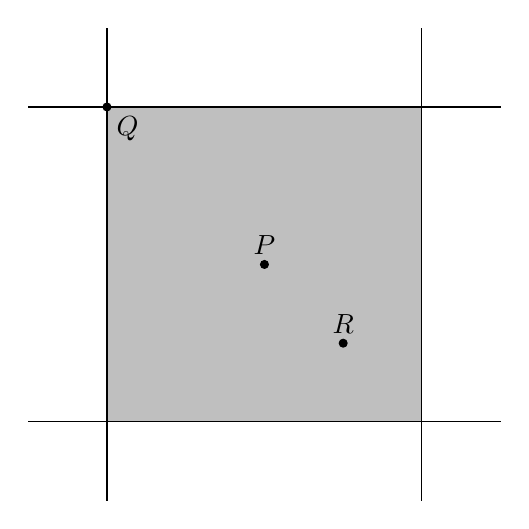
\begin{tikzpicture}
  \fill[gray!50] (0,0) rectangle (4,4);
  \draw (-1,-1) grid[xstep=4cm,ystep=4cm] (5,5);
  
  \draw[fill=black] (2,2) circle [radius=0.05cm] node[above] {$P$};
  \draw[fill=black] (0,4) circle [radius=0.05cm] node[anchor=north west] {$Q$};
  \draw[fill=black] (3,1) circle [radius=0.05cm] node[above] {$R$};
\end{tikzpicture}

\end{document}